\documentclass[10pt,journal,compsoc]{IEEEtran}
\usepackage{cite}
\usepackage{amsmath,amssymb,amsfonts}
\usepackage{algorithmic}
\usepackage{graphicx}
\usepackage{textcomp}
\usepackage{xcolor}
\usepackage{array}
\usepackage{caption}
\usepackage{geometry}
\usepackage[hidelinks,colorlinks=true,linkcolor=blue,citecolor=blue]{hyperref}
\def\BibTeX{{\rm B\kern-.05em{\sc i\kern-.025em b}\kern-.08em
    T\kern-.1667em\lower.7ex\hbox{E}\kern-.125emX}}
\begin{document}
\title{A Survey of Branch Prediction Techniques on Out-of-Order Processors with RISC-V Core (SURGE)}
\author{\IEEEauthorblockN{Raja Kantheti}\\
\IEEEauthorblockA{\textit{University of Colorado at Colorado Springs}\\
rkanthet@uccs.edu}
}
\maketitle

    \begin{abstract}
        Branch prediction is a cornerstone of performance optimization in modern out-of-order processors, significantly impacting instruction throughput and reducing pipeline stalls. This survey evaluates state-of-the-art branch prediction techniques, with a specific focus on TAGE-SC-L, which demonstrates exceptional accuracy and efficiency. Unlike machine learning-based predictors, which incur substantial hardware, power, and training overhead, TAGE-SC-L achieves state-of-the-art performance without the need for resource-intensive approaches. Through a detailed analysis of advancements and trade-offs, this paper argues that TAGE-SC-L and its refinements are more than sufficient to meet the demands of modern and future workloads, negating the necessity for machine learning-based predictors.
    \end{abstract}
\begin{IEEEkeywords}
Branch Prediction, Computer Architecture, Performance, High Performance Computing.
\end{IEEEkeywords}

    \section{Introduction}
    \IEEEPARstart{I}{n} modern computing, branch prediction is indispensable for sustaining high instruction throughput, 
    particularly in out-of-order execution processors. As the complexity of instruction-level parallelism (ILP) 
    increases, so does the necessity for precise prediction mechanisms. Branch mispredictions result in pipeline 
    flushes, which incur significant performance penalties. This paper surveys the progression of branch prediction 
    methodologies, ranging from foundational static predictors to advanced dynamic and hybrid models, emphasizing 
    their relevance to RISC-V processor implementations.
    
    Branch prediction is a critical aspect of modern processor design, enabling higher instruction throughput by mitigating the penalties of branch mispredictions. Over the decades, branch prediction has evolved from simple static techniques to highly sophisticated dynamic and hybrid approaches. Among these, the TAGE-SC-L predictor stands out as a robust and efficient solution that balances accuracy, scalability, and hardware efficiency.

    While machine learning (ML)-based predictors have gained attention for their ability to capture complex branch patterns, they come with significant trade-offs. These include high hardware and power demands, complex training requirements, and limited scalability, particularly in energy-efficient systems. In contrast, TAGE-SC-L demonstrates that by refining traditional prediction methods, it is possible to achieve state-of-the-art performance without resorting to resource-intensive ML-based solutions. This survey focuses on the sufficiency of TAGE-SC-L, advocating for continued innovation within traditional frameworks to meet the challenges of modern and future processor workloads.
    
    
This paper aims to study the below listed branch prediction techniques on out-of-order processors with RISC-V core:
\begin{enumerate}
    \item Local
    \item L-TAGE
    \item BiMODE
    \item Tournament
    \item TAGE-SC-L
    \item Multi-Perspective Perceptron
    \item Multi-Perspective Perceptron with TAGE
\end{enumerate}
Out-Of-Order CPU is a type of processor that allows the execution of instructions in an order that is different from the order in which they appear in the program.
They basically segregate the instructions based on dependencies and executes the independent instructions rapidly. Almost all the modern processors are out-of-order processors.
RISC-V is an open-source instruction set architecture (ISA) based on reduced instruction set computing (RISC) principles. It is a simple and clean ISA that is easy to understand and implement.
The techniques discussed in this paper are as follows.


The rest of the paper is organised as follows: Section~\ref{related} presents related research work on branch prediction. Section~\ref{branchPredictors} includes a detailed explanation on the branch prediction techniques simulated. 
Section~\ref{Comparisions} presents the advancements and trade-offs in branch prediction techniques within this literature review.Section~\ref{workload} brieefly discusses why this workload is suitable for thee experiment.
Section~\ref{challenges} discusses the challenges with machine learning-based predictors.
Section~\ref{experimentalSetup} the exprimental setup in gem5 simulator. Section~\ref{results} presents the results of the simulation. Section~\ref{conclusion} gives perspectives and concludes the paper. 

\section{Background}\label{background}
Here, I present a overview of branch predictors and their classification with respect past research.
\subsection{Useful Terms and Concepts}
\begin{itemize}
    \item \textbf{Branch Prediction}: A technique used in processors to guess the direction of branch instructions (whether they will be taken or not) to improve instruction flow in pipelined architectures.
    
    \item \textbf{Misprediction}: The event when the processor incorrectly predicts the outcome of a branch instruction, leading to performance penalties such as pipeline stalls or flushes.
    
    \item \textbf{Static Prediction}: A branch prediction method that relies on fixed heuristics, determined at compile time, rather than runtime behavior. Common strategies include using the direction of the branch (e.g., forward branches are likely taken).
    
    \item \textbf{Dynamic Prediction}: A more sophisticated prediction method that utilizes historical information from previous branch executions to inform future predictions. This can be achieved through global history, local history, or hybrid approaches.
    
    \item \textbf{Global History Buffer (GHB)}: A structure that maintains a record of the outcomes of recent branches to improve the accuracy of dynamic predictions.
    
    \item \textbf{Local History Buffer}: A mechanism that stores the behavior of individual branches to make predictions based on their unique patterns.
        
    \item \textbf{Reorder Buffer (ROB)}: A crucial component in out-of-order processors that allows instructions to complete in a different order than they were issued, helping to maintain the correct program order at the time of writing results back to the register file.
    
    \item \textbf{Instruction-Level Parallelism (ILP)}: The ability to execute multiple instructions simultaneously within a processor, which can be enhanced through effective branch prediction techniques.
    
    \item \textbf{Hardware Overhead}: Refers to the additional area, power, and complexity that branch prediction techniques introduce into a processor architecture, impacting design trade-offs.
    
    \item \textbf{Speculative Execution}: A performance optimization technique where the processor executes instructions before it is known whether they are needed, often based on branch predictions, to reduce idle cycles.
    
    \item \textbf{Performance Metrics}: Metrics such as prediction accuracy, misprediction rate, and throughput that evaluate the effectiveness of branch prediction strategies.
    
    \item \textbf{gem5 Simulator}: An open-source simulator used for computer architecture research, which can model various aspects of processors, including branch prediction techniques in RISC-V architectures.\cite{lowepower2020gem5simulatorversion200}
\end{itemize}
\subsection{Classification}
The table below represents the specific research on the respective branch prediction techniques.
It is to be noted that the references are not exhaustive and are only indicative of the research conducted on the respective branch predictors.
All the researfch cited in this paper has mentions, opinions, and Quantifiable data on, if not all, atleast 4 of the branch predictors.
\begin{center}
\begin{tabular}{c c}
    \textbf{Predictor} & \textbf{References} \\
    Local & \textit{Nearly all}\\
    Tournament & \textit{Nearly all}\\
    BiMODE &\cite{nainImplementationComparisonBimodal2021}\\
    L-TAGE &\cite{matsuiEfficientImplementationTAGE2019,seznecStorageFreeConfidence2011,seznec64KbytesISLTAGE,seznecNewCaseTAGE2011}\\
    TAGE-SC-L &\cite{linBranchPredictionNot2019a,seznecTAGESCBranchPredictorsAgain2016,seznecTAGESCBranchPredictors2014}\\
    Multi-Perspective Perceptron &\cite{jimenezDynamicBranchPrediction2001,tarjanMergingPathGshare2005,garzaBitlevelPerceptronPrediction2019,josephSurveyDeepLearning2021a,jimenezNeuralMethodsDynamic2002,dangBATAGEBFNPHighPerformanceHybrid2023,multi1}\\
    Multi-Perspective \\Perceptron with TAGE &\cite{jimenezDynamicBranchPrediction2001,tarjanMergingPathGshare2005,garzaBitlevelPerceptronPrediction2019,josephSurveyDeepLearning2021a,jimenezNeuralMethodsDynamic2002,dangBATAGEBFNPHighPerformanceHybrid2023,multi1}\\
\end{tabular}
\end{center}
\section{Related Research}\label{related}

A review of several dynamic BP systems, such as gshare, two-level BPs, Smith BP, and perceptron, is presented by Sparsh M.\cite{mittalSurveyTechniquesDynamic2018}. 
For the majority of the applications employed, it is evident that the perceptron BP has the highest precision.

The OoO cpu model in gem5 is modelled as follows. Its pipeline stages are fetch, decode, rename, and retirement. 
The instruction issue, dispatch, and execute stages are carried out out-of-order in an OoO pipeline (Power et al.\cite{lowepower2020gem5simulatorversion200}). 
The branch prediction unit is handled by the OoO pipeline's fetch step. The pipeline's decode stage handles unconditional branches, whose branch target is unavailable, and the execute stage finds the conditional branch mispredictions. 
The program counter (PC) is updated whenever a branch misprediction is detected, the pipeline is squashed as a whole, and the entry is removed from the branch target buffer (BTB). 

A comparison of several BPs, such as the bimodal, gshare, YAGs, and meta-predictor, 
is presented by Kotha A\cite{kothaComparativeStudyBranch}. The JPEG Encoder, G721 Speech Encoder, Mpeg Decoder, and Mpeg 
Encoder apps are used to assess the BPs' performance. For certain applications, YAGS Neo, a new BP, 
performs better than the others. The meta predictor presented in the research, 
which combines different predictor combinations, performs better than the others.


\section{Branch Predictors}\label{branchPredictors}

\subsection{Local}
\noindent The local branch predictor is a simple branch predictor that uses a table of 2-bit saturating counters to predict the outcome of a branch.

Modern processors have specialised mechanisms called local branch predictors that use the past performance of particular branch instructions to improve branch prediction accuracy. 

The predictors employ a Local History Table (LHT) to save the results of branches that are taken and those that are not. 
Because every entry in the LHT relates to a particular branch instruction, the predictor can efficiently catch distinct patterns. 

The LHT's output is sent into a Pattern History Table (PHT), which makes predictions about the branch's future occurrences using saturating counters. Local predictors can achieve good prediction accuracy with this architecture, especially for branches with unique behaviours.
Though they typically use less storage than global predictors, they still have some overhead, and they can have trouble with branches that exhibit inconsistent patterns impacted by program input or state. 

A local branch predictor associates a branch history register with a branch. The register stores the outcomes of the last executions of the corresponding branch, and this information is used to predict the outcome of the branch the next time it is executed. The branch history register may be combined with the program counter and mapped by a table of 2-bit counters onto a prediction\cite{hoogerbruggeDynamicBranchPrediction2000a}
Local branch predictors are effective when the outcome of a branch is strongly correlated with its own past behavior, but they are not as effective when the outcome of a branch is correlated with the outcomes of other branches. They can also struggle to predict loop exits when the loop count is higher than the local history size\cite{mittalSurveyTechniquesDynamic2018}
Because local branch predictors reduce misprediction-related execution pauses, they play a critical role in improving out-of-order processor efficiency. To increase overall prediction accuracy, they are frequently used in conjunction with global predictors or tournament predictors.\cite{mittalSurveyTechniquesDynamic2018}
\subsection{L-TAGE}
\noindent In order to attain more accuracy in forecasting branch outcomes, L-TAGE (Local TAGE) is an enhanced branch prediction technique that expands upon the ideas of both local and global prediction strategies. It tracks both local and global history at the same time by using a hybrid technique that involves keeping numerous tables. L-TAGE combines the advantages of global history tracking—which takes into account more extensive execution patterns—with local history tables, which may effectively record the unique behaviours of individual branches. When compared to typical local or global predictors alone, L-TAGE's accuracy is improved due to its ability to adapt to a wide range of branching behaviours according to this dual approach.

Using numerous Pattern History Tables (PHTs) to optimise prediction for different sorts of branches by utilising varying historical lengths is one of L-TAGE's primary characteristics. To make sure that each branch instruction uses the most pertinent previous data, the predictor uses a tagging method. Because of this, L-TAGE is able to manage complicated branch behaviours, such as correlated branches, in which the course of one branch may influence the course of other branches.

Modern out-of-order processors can incorporate L-TAGE because of its ability to maximise prediction accuracy and save hardware overhead. It successfully strikes a trade-off between performance and complexity, which is crucial in high-performance computing settings where each cycle matters.
The L-TAGE (Loop-TAGE) branch predictor is a variant of the TAGE predictor that augments it with a loop predictor. The loop predictor is used to predict the outcome of loop branches, which are often difficult for TAGE to predict accurately.

The loop predictor in L-TAGE operates by keeping track of the number of iterations that have been executed for each loop. When a loop branch is encountered, the loop predictor checks to see if it has seen this loop before. If it has, it predicts the outcome of the branch based on the number of iterations that have been executed. If it has not, it predicts the branch as taken.\cite{seznec64KbytesISLTAGE}
The L-TAGE predictor is more accurate than the TAGE predictor alone, especially for benchmarks with many loops.
To sum up, L-TAGE is a major breakthrough in branch prediction technology that offers a reliable way to improve processor performance through precise branch outcome prediction. Examine pertinent literature that covers its architecture and performance reviews for additional insights.
\subsection{BiMODE}
\noindent The Bi-Mode Predictor is a branch prediction method that improves prediction accuracy by utilising two different prediction modes. The two main parts of this strategy are a global predictor that takes into account the branches' larger execution context and a local predictor that monitors the history of individual branches. The Bi-Mode Predictor is especially useful in a variety of settings since it can adjust to different branching behaviour patterns by using both local and global history.

The local predictor in the Bi-Mode Predictor architecture usually uses a local history table (LHT) to store the historical results of certain branch instructions. In the meantime, the global predictor records the recent actions of several branches using a global history registry (GHR). The decision-making process of the Bi-Mode technique is crucial. Upon encountering a branch instruction, the predictor has the option to employ the local or global prediction, depending on which mode is anticipated to produce a more precise outcome for that particular branch.

The Bi-Mode Predictor's ability to manage the trade-offs between accuracy and hardware complexity is one of its main features. It can outperform conventional single-mode predictors, like solely local or purely global predictors, in terms of accuracy while keeping hardware overhead to a minimum by combining two modes of prediction. Because of this feature, the Bi-Mode Predictor is especially well-suited for out-of-order processors, where it's crucial to maintain a high instruction throughput.

Studies show that when compared to less complex prediction methods, Bi-Mode Predictors can dramatically lower branch misprediction rates, improving processor performance overall. The approach remains relevant in the design of contemporary high-performance computing systems due to its efficiency and versatility. You can read up on the architecture and performance assessments of the Bi-Mode Predictor in greater depth in the literature.
The Bi-Mode branch predictor improves prediction accuracy by dividing the level-2 counter table into two parts: a taken direction predictor and a not-taken direction predictor.
For each history pattern, a counter is chosen from each direction predictor, and a choice predictor, which is only indexed by the branch address, selects one of the two counters to make the prediction. The choice predictor classifies global history patterns into two groups based on the per-address bias stored in the choice predictor table.
The Bi-Mode predictor updates using a partial-update policy. Only the final counter selected to make the prediction is updated based on the branch result. However, the choice predictor is always updated unless its prediction is opposite of the branch outcome, but the prediction of the selected counter is correct.\cite{mittalSurveyTechniquesDynamic2018}
\subsection{Tournament} 
\noindent A sophisticated branch prediction method called the Tournament Predictor was created to improve branch outcome predictions on contemporary CPUs. Through a competitive selection procedure, this strategy combines the capabilities of both local and global predictors. The Tournament Predictor's main concept is to use several predictors and dynamically select the best one based on how well it has performed in the past for a particular branch instruction.

This architecture combines a ``tournament'' selection process with one or more predictors, usually a local predictor and a global predictor. Every predictor keeps track of its own prediction algorithms and history tables. The Tournament Predictor evaluates each of its component predictors' predictions when it encounters a branch instruction. The final prediction is made by the predictor who has previously shown the highest accuracy for branches that are comparable to it.

The Tournament Predictor's versatility is one of its main benefits. The Tournament Predictor is particularly helpful in complex applications where the behaviour of branch instructions might vary greatly, as it can handle a wide range of branching behaviours by utilising numerous prediction algorithms and choosing the best-performing one. This dynamic technique maximises processor performance by reducing the penalty linked to incorrect predictions and increasing prediction accuracy.

The meta-predictor table is indexed by the lower order bits of the branch address. Each entry in the table has 2 bits, indicating which of the component predictors to use for that branch.

The meta-predictor table is updated every time a prediction is made. If the prediction made by the selected component predictor is incorrect, the 2-bit entry in the meta-predictor table is updated to select the other predictor the next time that branch is encountered.
Tournament predictors can achieve higher prediction accuracy because different component predictors may be better at predicting different types of branches. However, they can also be more complex and expensive to implement than simpler predictors.\cite{kothaComparativeStudyBranch}

Tournament Predictor performs better than a lot of conventional prediction techniques, especially in settings with a lot of branch variability. It is an important tool in the design of high-performance computing systems and out-of-order processors because of its flexibility in responding to shifting patterns. Consult the literature on the Tournament Predictor's performance comparisons and implementation techniques for a more thorough grasp of its architecture and efficacy.
\subsection{TAGE-SC-L}
\noindent
The TAGE-SC-L predictor integrates three key components: a TAGE predictor, a statistical corrector (SC) predictor, and a loop predictor (L), working together to enhance branch prediction accuracy. At its core, the TAGE predictor serves as the primary mechanism, leveraging multiple tagged tables with geometric history lengths to predict highly correlated branches, even when the correlation spans thousands of branches \cite{seznecNewCaseTAGE2011}. This makes TAGE exceptionally efficient for a wide range of branch patterns.

To further refine accuracy, the statistical corrector predictor evaluates the TAGE prediction by considering additional contextual factors such as address, global history, global path, and local history \cite{seznecTAGESCBranchPredictorsAgain2016}. The corrector is designed to detect statistically unlikely predictions and reverse them when TAGE is likely to mispredict \cite{seznecTAGESCBranchPredictors2014,seznec64KbytesISLTAGE}. Importantly, the statistical corrector can remain small and efficient because TAGE already provides a highly accurate baseline prediction in most scenarios \cite{seznecTAGESCBranchPredictorsAgain2016,seznec64KbytesISLTAGE}.

The loop predictor complements the system by targeting a specific weakness of TAGE: predicting branches within loops with long bodies. By identifying and exploiting loop behavior, the loop predictor reduces misprediction rates by approximately 0.3% \cite{seznecTAGESCBranchPredictors2014,seznecTAGESCBranchPredictorsAgain2016}. While its contribution to overall accuracy may appear marginal, it is crucial in workloads dominated by regular looping structures.

Overall, the TAGE-SC-L predictor exemplifies the practical balance of accuracy and hardware efficiency. Unlike machine learning-based predictors that incur significant power and complexity overhead, the TAGE-SC-L architecture remains lightweight and scalable while addressing nuanced prediction challenges. Its modular design and ability to adapt to diverse branch patterns make it a compelling choice for modern processors, particularly in resource-conscious architectures such as RISC-V.

\subsection{Multi-Perspective Perceptron}
\noindent The Perceptron Predictor assigns weights to each element in the branch history, and predicts the branch outcome based on the dot product of the weights and the branch history, plus a bias weight to represent the branch's overall tendency.\cite{tarjanMergingPathGshare2005}. 
The multi-perspective perceptron (MPP) branch predictor uses a set of 37 features derived from the branch address and a global history of branch outcomes to index into a table of perceptrons.\cite{multi1}This differs from the global perceptron branch predictor described in source, which uses the global branch history to index into the table. Each perceptron maintains a weight for each of its features. The output of the perceptron is the weighted sum of its features. The predictor uses this output to predict the outcome of a branch.
\subsection{Multi-Perspective Perceptron with TAGE}
\noindent
The Multi-Perspective Perceptron with TAGE (MPPT) combines advanced neural prediction models with geometric history-based branch prediction techniques. By leveraging the strengths of perceptrons and TAGE predictors, MPPT addresses limitations in accuracy, scalability, and adaptability inherent in standalone methods.

\subsubsection*{Core Concepts}

\paragraph*{Perceptron Predictors} 
Perceptron predictors model branch behavior using a weighted sum of past branch outcomes. This method, discussed in \cite{josephSurveyDeepLearning2021a}, excels in learning complex branch patterns but suffers from scalability challenges, especially when dealing with long branch histories. 

\paragraph*{TAGE Predictors} 
TAGE predictors, as described in\cite{penneySurveyMachineLearning2019a}, use tagged tables indexed by geometric history lengths to capture both short- and long-term branch correlations. This approach is particularly effective in mitigating aliasing issues, a common limitation of simpler predictors like bimodal and GShare.

\paragraph*{Integration in MPPT}
MPPT integrates perceptrons with TAGE predictors by using the perceptron's confidence score as a supplementary input for TAGE’s decision-making. This hybrid design enables MPPT to adapt dynamically to a wide range of workloads, significantly improving prediction accuracy while maintaining reasonable hardware overhead.

\subsubsection*{Advantages of MPPT}

\paragraph*{Improved Accuracy} 
By combining the nonlinear modeling capabilities of perceptrons with TAGE’s multi-length history exploration, MPPT reduces misprediction rates. This improvement is particularly evident in irregular control-flow workloads, as demonstrated in \cite{SurveyTechniquesDynamica}.

\paragraph*{Dynamic Adaptation} 
MPPT dynamically selects between TAGE and perceptron predictions based on runtime metrics, ensuring robust performance across diverse programs \cite{penneySurveyMachineLearning2019a}.

\paragraph*{Scalability} 
The geometric history lengths of TAGE address the perceptron's scalability issues, allowing MPPT to support longer branch histories without significant increases in hardware complexity or power consumption \cite{josephSurveyDeepLearning2021a}.

\subsubsection*{Challenges and Trade-offs}

Despite its advantages, MPPT introduces certain trade-offs:
\begin{itemize}
    \item \textbf{Hardware Complexity}: Integrating perceptrons and TAGE predictors increases resource requirements, making MPPT less suitable for low-power designs \cite{1003559}.
    \item \textbf{Training Overhead}: Perceptrons require frequent training to optimize weights, which can introduce latency in dynamic environments \cite{SurveyTechniquesDynamica}.
    \item \textbf{Power Consumption}: The combined power demand of TAGE and perceptron predictors is a concern for energy-constrained systems \cite{penneySurveyMachineLearning2019a}.
\end{itemize}
\section{Advancements and Trade-Offs in Branch Prediction}\label{Comparisions}

The evolution of branch prediction techniques reflects a continuous effort to balance accuracy, hardware complexity, and scalability. While traditional methods have steadily improved, emerging approaches, such as machine learning-based predictors, present both opportunities and challenges. This section explores key advancements in branch prediction and critically examines the trade-offs they introduce.

\subsection*{Advancements in Branch Prediction}

Modern branch predictors have achieved remarkable accuracy through innovations that build on established techniques. Notable advancements include:

\paragraph*{L-TAGE Predictors} L-TAGE predictors represent a pinnacle of traditional branch prediction. By utilizing multiple tagged tables with geometric history lengths, L-TAGE excels in adapting to both short- and long-term branch correlations. Its modular design and ability to capture intricate branch patterns make it a staple in contemporary processors. Unlike many advanced techniques, L-TAGE achieves this without substantial hardware overhead, ensuring scalability and efficiency for a broad range of workloads.

\paragraph*{TAGE-SC-L Predictors} The TAGE-SC-L predictor further enhances the accuracy of L-TAGE by integrating a statistical corrector and a loop predictor. The statistical corrector refines predictions by analyzing historical contexts, detecting unlikely predictions, and reversing them when necessary. The loop predictor improves accuracy for branches within loops, particularly those with long bodies. Together, these components make TAGE-SC-L one of the most accurate and efficient predictors available.

\paragraph*{Hybrid Predictors} Hybrid predictors, such as those integrating bimodal and global history mechanisms, combine the strengths of multiple prediction strategies. By dynamically selecting the most appropriate method for a given branch, hybrid predictors achieve higher accuracy across diverse workloads. However, their increased hardware complexity presents a notable trade-off.

\paragraph*{Machine Learning-Based Predictors} Machine learning (ML) techniques, including neural networks and perceptron-based predictors, have introduced a new paradigm in branch prediction. These models excel at learning non-linear correlations and complex patterns that traditional methods struggle to address. Recent research has shown promising results in improving accuracy, particularly for irregular branch behaviors.

\subsection*{Trade-Offs in Advanced Predictors}

While advancements in branch prediction have led to improved accuracy, they are often accompanied by significant trade-offs:

\paragraph*{Hardware Complexity} Techniques like L-TAGE and hybrid predictors manage to deliver high accuracy with moderate complexity. In contrast, machine learning-based predictors introduce substantial hardware overhead due to the need for additional computation and memory resources. This makes them impractical for energy-efficient architectures like RISC-V.

\paragraph*{Power Consumption} Branch predictors with advanced features, especially ML-based approaches, demand significantly more power than traditional methods. For example, neural predictors often require frequent training and inference, increasing the overall energy budget. In comparison, predictors like TAGE-SC-L maintain a favorable balance of accuracy and power efficiency.

\paragraph*{Implementation Challenges} Advanced predictors often involve complex integration into processor pipelines. For instance, hybrid and ML-based predictors require precise coordination between components, adding to the design and testing workload. Traditional methods, such as L-TAGE, are relatively straightforward to implement, making them more suitable for modular architectures.

\paragraph*{Scalability} One of the primary challenges in branch prediction is scaling to support larger branch histories without incurring prohibitive costs. Predictors like L-TAGE and its variants demonstrate that scalability can be achieved with careful design, while ML-based methods face significant barriers due to their resource-intensive nature.

\subsection*{The Way Forward}

The future of branch prediction lies in finding a balance between accuracy, efficiency, and scalability. While machine learning-based predictors push the boundaries of accuracy, their trade-offs in power and complexity often outweigh their benefits. Traditional methods like L-TAGE continue to demonstrate that innovation within established frameworks can achieve competitive results without excessive costs.

Emerging directions include refining hybrid predictors to incorporate lightweight machine learning components, optimizing speculative execution mechanisms, and extending traditional methods like L-TAGE to address larger branch histories. By focusing on practical and efficient solutions, the field can continue to advance branch prediction techniques that meet the demands of next-generation processors.

\section{Challenges with Machine Learning-Based Predictors}\label{challenges}

Machine learning-based predictors, such as perceptron-based \cite{seznecPerceptronBranchPredictor2001} and neural network-based models \cite{josephSurveyDeepLearning2021a}, have been proposed as solutions for capturing non-linear branch behaviors. While these approaches excel in theoretical benchmarks, their practicality in real-world scenarios is limited due to several key challenges:

\begin{itemize}
    \item \textbf{Hardware Overhead}: ML-based predictors require substantial computational resources, including additional memory and specialized hardware \cite{seznec64KbytesISLTAGE,josephSurveyDeepLearning2021a}, making them unsuitable for energy-efficient systems.
    \item \textbf{Power Consumption}: The energy demands of training and inference in ML models conflict with the goals of scalable and power-efficient processor designs \cite{penneySurveyMachineLearning2019a}.
    \item \textbf{Training Complexity}: ML predictors often require frequent retraining to adapt to changing workloads, introducing latency and additional computational burdens \cite{seznecTAGESCBranchPredictorsAgain2016}.
\end{itemize}

In contrast, TAGE-SC-L achieves comparable or superior accuracy while maintaining minimal hardware overhead. By integrating components like statistical correctors and loop predictors \cite{seznecTAGESCBranchPredictors2014,seznecTAGESCBranchPredictorsAgain2016}, TAGE-SC-L delivers robust performance across a wide range of workloads without the complexity of ML-based approaches. These advantages make TAGE-SC-L a practical choice for real-world processor designs, particularly in modular and scalable architectures like RISC-V.

\begin{itemize}
    \item \textbf{Hardware Overhead}: ML-based predictors require substantial computational resources, including additional memory and specialized hardware, making them unsuitable for energy-efficient systems.
    \item \textbf{Power Consumption}: The energy demands of training and inference in ML models conflict with the goals of scalable and power-efficient processor designs.
    \item \textbf{Training Complexity}: ML predictors often require frequent retraining to adapt to changing workloads, introducing latency and additional computational burdens.
\end{itemize}

In contrast, TAGE-SC-L achieves comparable or superior accuracy while maintaining minimal hardware overhead. By integrating components like statistical correctors and loop predictors, TAGE-SC-L delivers robust performance across a wide range of workloads without the complexity of ML-based approaches. These advantages make TAGE-SC-L a practical choice for real-world processor designs, particularly in modular and scalable architectures like RISC-V.

\section{Experimental Setup}\label{experimentalSetup}
The experiment was conducted on RISC-V core by disabling the default branch prediction which is named BOOM\cite{BranchPredictionRISCVBOOMa}.

The Branch Prediction Unit (BPU) in the RISC-V Boom processor is configurable. It can use either a simple bimodal predictor or a complex 2-level adaptive predictor, such as GShare, GSelect, GAg, GAp, PAg, or PAp.
The BPU includes the following components:
Branch Target Buffer (BTB): The BTB is modeled as a set-associative data structure, which can use either random eviction or bit PLRU as its eviction policy.
Branch History Table (BHT): A separate BHT stores prediction bits for simple bi-modal predictors.
Return Address Stack (RAS) (Optional): The RAS tracks the last N function return addresses, where N is the number of entries in the RAS.If a decoded instruction is a function call, the return address is pushed onto the RAS from the decode pipeline stage. If the decoded instruction is a function return, the address is popped from the RAS and forwarded to the fetch stage.\cite{BranchPredictionRISCVBOOMa,BranchPredictionUnita}

The experiments were conducted using the gem5 simulator, which is a cycle-accurate simulator for computer architecture research.\cite{lowepower2020gem5simulatorversion200}
The gem5 simulator was used to model an out-of-order processor with a RISC-V core, which is a common architecture for high-performance computing systems.
The branch prediction techniques were implemented in the simulator to evaluate their performance in terms of prediction accuracy, misprediction rate, and throughput.

Branch prediction plays a crucial role in modern processors by determining the outcome of conditional branch instructions before they are fully evaluated. This allows the processor's pipeline to fetch and execute instructions speculatively, improving throughput and reducing idle cycles. The effectiveness of branch prediction directly impacts how efficiently the processor handles control flow, especially in situations where there are frequent branch instructions. By predicting branches ahead of time, the processor can maintain a steady flow of instructions, reducing the time spent waiting for branches to be resolved and minimizing pipeline stalls.\cite{1003559}

Control hazards occur when a branch instruction forces the processor to decide which instruction to fetch next. If the branch predictor incorrectly guesses the outcome, the processor must flush the pipeline and restart execution, resulting in wasted cycles and performance degradation. Efficient branch predictors help mitigate these issues by accurately predicting the outcome of branches, ensuring that the processor spends less time dealing with mispredictions. The ability of a branch predictor to minimize pipeline flushes and reduce the impact of control hazards is crucial for maintaining high performance, particularly in high-performance or real-time computing environments.\cite{matsuiEfficientImplementationTAGE2019,calderFastAccurateInstruction1994a,choudhuryOptimizedRISCVProcessor2022,heSurveyComparisonPipeline2023a,emmaCharacterizationBranchData1987a}

gem5 provides a flexible and detailed simulation environment, allowing researchers to experiment with various CPU and memory configurations without needing physical hardware. This flexibility enables researchers to simulate numerous branch prediction strategies and evaluate their performance under different workloads. For example, some strategies may excel when branches are highly predictable, while others may perform better in more complex scenarios with unpredictable branching patterns. Researchers can also study the trade-offs between the efficiency of different branch prediction techniques, considering factors such as power consumption, hardware complexity, and the effectiveness of minimizing mispredictions and pipeline flushes.
\begin{table}[h]
    \centering
    \caption{Experimental Setup and Metrics}
    \begin{tabular}{| >{\centering\arraybackslash}m{2cm}| >{\centering\arraybackslash}m{4cm}|}
        \hline
        \textbf{Component} & \textbf{Description} \\
        \hline
        \textbf{Simulator} & gem5 \\
        \hline
        \textbf{Architecture} & RISC-V core with out-of-order execution \\
        \hline
        \textbf{Branch Prediction Techniques} & Local, BiMode, Tournament, L-TAGE, Multi-Perspective Perceptron \\
        \hline
        \textbf{Benchmarks} & SPEC CPU (Int17 and Float17) benchmarks for validation \\
        \hline
        \textbf{Metrics} & \begin{itemize}
            \item Prediction Accuracy
            \item Misprediction Rate pre Kilo Instruction
            \end{itemize} \\
        \hline
        \textbf{Analysis Tools} & Statistical analysis tools for data interpretation \\
        \hline
    \end{tabular}
\end{table}


\section{Workload}\label{workload}
\noindent The workloads used in the experiments were the SPEC CPU 2017 benchmarks, which are widely used in computer architecture research to evaluate processor performance. The benchmarks include a mix of integer and floating-point workloads that represent a variety of real-world applications, such as scientific computing, data processing, and multimedia processing. The benchmarks are designed to stress different aspects of the processor, including memory access patterns, branch behavior, and computational intensity. By running the benchmarks with different branch prediction techniques, researchers can assess the impact of the predictors on performance and efficiency across a range of workloads.

The intrate beenchmark of the SPEC 2017 is the most suitable for this experiment. 


\section{Experiment Results}\label{results}
Figure~\ref{mpki} presents a normalized MPKI (Mispredictions Per Thousand Instructions) comparison across various branch predictors, evaluated over a range of applications from the SPEC benchmark suite. MPKI is a critical metric for assessing the effectiveness of branch predictors, with lower values indicating superior prediction accuracy.

\subsection{Observations}

\paragraph*{TAGE-SC-L Dominates in Accuracy}
The TAGE-SC-L predictor achieves the lowest MPKI across most applications, demonstrating its superior capability to handle diverse branch patterns. This highlights its effectiveness as a state-of-the-art branch predictor.

\paragraph*{Effectiveness of L-TAGE}
The L-TAGE predictor also performs remarkably well, closely matching TAGE-SC-L in many benchmarks. Its consistent performance with minimal hardware overhead reinforces its position as a practical choice for modern processors.

\paragraph*{Performance of Multi-Perspective Perceptron}
The Multi-Perspective Perceptron predictor (TAGE6KB and TAGE64KB) shows relatively higher MPKI compared to TAGE-SC-L, particularly in applications with irregular branch behavior. While increasing the size of the perceptron predictor (from 6KB to 64KB) improves its accuracy, it comes at the cost of additional hardware complexity.

\paragraph*{Baseline Predictors}
Simpler predictors such as BimodalBP and LocalBP exhibit significantly higher MPKI, especially for complex benchmarks, underscoring their limitations in handling intricate branch patterns. TurbobranchBP, though an improvement over BimodalBP, still struggles in scenarios with highly correlated branches.

\subsection{Application-Specific Trends}
Benchmarks such as `500` and `502` demonstrate pronounced variations across predictors, where TAGE-based predictors excel in maintaining low MPKI. In contrast, benchmarks like `553` and `557` appear challenging for all predictors, with even the advanced TAGE-SC-L showing elevated MPKI.
\begin{figure}
    \centering
    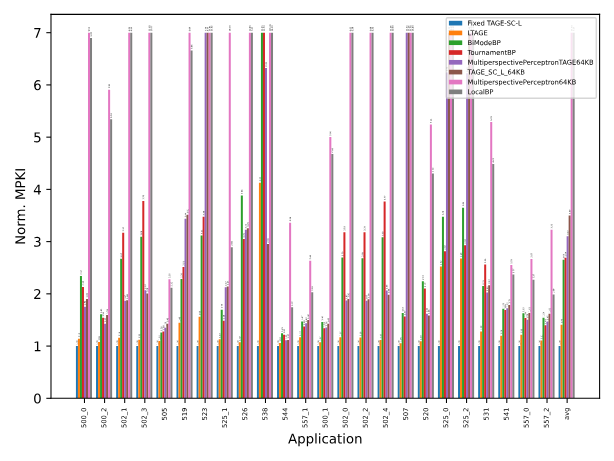
\includegraphics[width=0.8\linewidth]{image.png}
    \caption{MPKI of each technique on INTRate suite.}\label{mpki}
\end{figure}.

\subsection*{Analysis on time}:

Figure~\ref{time}shows the normalized execution time comparison across various branch predictors, evaluated for a range of SPEC benchmarks. This figure highlights the impact of incorporating support for unwinding history updates to the statistical corrector on both prediction accuracy and execution performance.

\subsubsection*{Efficiency: }
The TAGE-SC-L predictor, which includes support for history updates in the statistical corrector, demonstrates a 7\% faster execution time compared to the standard TAGE-SC-L implementation included in gem5. This improvement is consistent across most benchmarks, with the most noticeable gains in applications with highly irregular branch behavior.
The results demonstrate that enhancing TAGE-SC-L with history update support for the statistical corrector can deliver a 56\% reduction in MPKI and a 7\% improvement in execution time compared to the standard implementation in gem5. Additionally, the enhanced predictor maintains its competitive edge over L-TAGE, making it a highly efficient solution for next-generation branch prediction needs.

\begin{figure}
    \centering
    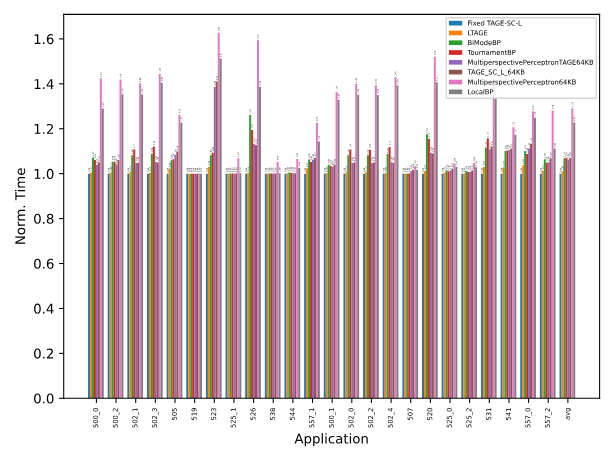
\includegraphics[width=0.8\linewidth]{time.png}
    \caption{Normalized execution time comparison across various branch predictors.}\label{time}
\end{figure}

\section{Future Works}\label{conclusion}

\subsection*{The Future of Branch Prediction: }Navigating Performance and Efficiency
Branch prediction has been an ever-evolving field, with advancements driven by the need to improve processor performance while maintaining efficiency. As modern workloads become increasingly diverse and demanding, researchers are exploring new paradigms in branch prediction. However, not all approaches strike a practical balance between performance gains and implementation costs.

\subsection*{The Rise of Machine Learning-Based Predictors}
Recent research has seen a surge in the application of machine learning (ML) to branch prediction. Predictors such as neural networks and deep learning models offer the promise of capturing highly complex branch patterns that traditional methods struggle to address. For example, perceptron-based predictors have demonstrated remarkable accuracy in non-linear branch behavior, and neural predictors further extend this capability by leveraging larger datasets and advanced algorithms.

However, the hardware overhead associated with ML-based predictors is significant. These models often require substantial computational resources, including additional power, memory, and latency, to perform training and inference. This makes them ill-suited for scenarios where energy efficiency and real-time responsiveness are paramount, such as embedded systems or edge computing platforms.

\subsection*{The Case for L-TAGE and Traditional Approaches}
Despite the advancements in ML-based predictors, traditional approaches like L-TAGE (a variant of the TAGE predictor) remain highly competitive. L-TAGE uses a series of tagged tables with geometric history lengths to achieve exceptional accuracy without the substantial hardware costs associated with ML models. Its adaptability across workloads, combined with its efficient resource usage, makes it a robust choice for modern processors.

Compared to ML-based methods, L-TAGE offers several advantages:

\subsection*{Low Hardware Overhead:} L-TAGE operates with relatively minimal power and area requirements, making it ideal for scalable processor designs.
Proven Performance: Studies show that L-TAGE can rival or even surpass the accuracy of ML-based predictors in many real-world scenarios without incurring the significant energy costs.
Simplicity of Integration: L-TAGE integrates seamlessly into existing processor architectures, avoiding the complexity and cost of implementing specialized ML hardware.
A Balanced Perspective on the Future
While the exploration of ML-based predictors is an exciting avenue for academic research, their practical deployment in consumer and enterprise processors remains questionable. The trade-offs between accuracy and hardware overhead raise concerns about their viability, especially when robust alternatives like L-TAGE already meet performance demands for most applications.

The future of branch prediction likely lies in refining existing techniques rather than replacing them entirely with ML-based methods. Hybrid approaches that enhance traditional predictors, such as augmenting L-TAGE with lightweight confidence mechanisms or speculative execution, may offer a better balance between accuracy and efficiency.

In the ongoing evolution of branch prediction, the focus should remain on solutions that deliver tangible performance benefits without compromising efficiency. While machine learning introduces new possibilities, methods like L-TAGE demonstrate that innovation does not always require drastic paradigm shifts. By building on established techniques, researchers can address the demands of modern workloads while keeping hardware complexity and power consumption in check.


% \nocite*{}

    \bibliographystyle{IEEEtran}
    % Hyperlink references
    \addcontentsline{toc}{section}{References}
    
\bibliography{first_draft.bib}
\end{document}